%!TEX root = ../dissertation.tex
\renewcommand{\chaptermark}[1]{\markboth{#1}{}}
\renewcommand{\sectionmark}[1]{\markright{#1}}
\fancyhead{} % clear all header fields
\fancyhead[LE]{\chaptername~\thechapter | \leftmark}
\fancyhead[RO]{\thesection~\rightmark}
\fancyfoot{} % clear all footer fields
\fancyfoot[LE,RO]{\thepage}

    
\chapter{Introduction}
\label{chp:intro}
%\epigraph{Oṃ bhūr buvaḥ svaḥ | tat savitur vareṇyaṃ | bhargo devasya dhīmahi | dhiyo yo naḥ pracodayāt}{Gāyatrī mantra}
%\epigraph{If I could remember the names of all these particles, I'd be a botanist.}{Enrico Fermi}
%\epigraph{Contemplator enim, cum solis lumina cumque inserti fundunt radii per opaca domorum: multa minuta modis multis per inane videbis corpora misceri radiorum lumine in ipso}{Lucretius, \textit{De Rerum Natura}}
\section{The dawn of the Sandard Model}
Understanding the fundamental constituents of matter and their interactions has been a central pursuit in the history of humanity. The first person who proposed the concept of ``Atomism" was the Greek philosopher Democritus, suggesting in the 6th century BC that all matter is composed of indivisible particles called atoms~\cite{laertius1853lives}.
%Empedocles also imagined fundamental elements and forces of attraction and repulsion allowing the elements to interact. 
This theory made its way in history along Epicurus and Plato, reaching Rome in the 1st century BC with Lucretius explaining it in the \textit{De Rerum Natura}~\cite{LucretiusCarus+2019}. 

With the decline of the Roman Empire and the rise of Scholasticism the atomic theory was abandoned for many ages. The 17th century, however saw a resurgence in the atomic theory primarily through the work on the corpuscular nature of light by Newton~\cite{Newton1704-NEWO}. From the early philosophical musings, the atomism theory entered the scientific world. The tight bond with the philosophical theory was highlighted in the 19th century by John Dalton. Through his work on stoichiometry, he concluded that each element of nature was composed of a single unique type of particle, naming this fundamental particle \textit{atom}~\cite{Dalton}. 

As physics entered the 20th century, it was discovered that atoms are not, in fact, the fundamental particles of nature, but are conglomerates of even smaller ``corpuscles". The experimental probe of the first corpuscle of matter was given by Thomson, who first observed the electrons in 1892~\cite{doi:10.1080/14786449708621070}. The atomic model subsequently was finally completed with the discovery of the constituents of the atomic nucleus: the proton (Rutherford 1919~\cite{doi:10.1080/14786440608635919}) and the neutron (Chadwick 1932~\cite{Chadwick:1932ma}). The observation of the photon by Compton in 1924~\cite{PhysRev.21.483, PhysRev.24.591} completed the picture of the stable matter observed in our universe, but a new field just opened: the study of subatomic particles. In this field, not only new constituents of matter were discovered, but also the interactions that govern them. In 1933, Enrico Fermi formulated a theory~\cite{Fermi:1934hr} of beta decays (a precursor of what will be called the weak interaction), while Yukawa in 1935 tried to provide a potential responsible for the strong interaction~\cite{Yukawa:1935xg}, that binds together the particles in the nucleus of the atom. 

The mid-20th century saw an explosion of particle discoveries, facilitated by the development of particle accelerators, which are complex machines that use electromagnetic fields to propel charged particles -- such as protons or electrons -- to high speeds. These accelerated particles are then made collide with each other or with stationary targets (made of atoms), enabling the interaction between the two at high energy. One of the first results of accelerator experiment was the discovery in 1955 of the antiproton~\cite{PhysRev.100.947}, i.e. a particle with the same mass but with opposite physical charges (such as electric charge). 

Particle accelerators such as colliders, enabled physicists to recreate the high-energy conditions of the early universe, allowing for the discovery of a plethora of new particles -- the ``subnuclear zoo" as called by Robert Oppenheimer~\cite{johnson2010strange} -- which eventually lead in the quark model proposed by Gell-Mann and Zweig in 1961~\cite{Gell-Mann:1964ewy}. In this new theory,  Gell-Mann and Zweig proposed the quarks as the fundamental elements of some type of particles called \textit{hadrons}. 

The quark model explains how quarks combine to form hadrons: baryons (such as protons and neutrons) are composed of three quarks, while mesons are composed of a quark and an antiquark pair.  This model not only provided a systematic way to categorise the myriad of hadrons discovered in particle accelerators but also predicted the existence of new particles, which were subsequently confirmed by experiments~\cite{PhysRevLett.12.204}. Quarks come in different types, known as ``flavors", and carry fractional electric charges. 

As the quark theory was first developed, only three flavours of quarks were assumed (up $u$, down $d$ and strange $s$). However, in 1970 the Glashow-Iliopoulos-Maiani (GIM) Mechanism~\cite{Glashow:1970gm} predicted the existence of a fourth quark (the charm), in order to explain why some transitions result suppressed. Of more importance, the GIM mechanism proposed that quarks are organised in a doublet-symmetry such as ($u,d$) ($c,s$). This theory was promptly extended in 1973 by Kobayashi and Maskawa~\cite{Kobayashi:1973fv} with a third generation of a doublet ($t,b$) made by a top and bottom quark. This extension was needed as the two physicists tried to generalise what was first theorised by Nicola Cabibbo, i.e. that there is a mixing between different flavours of quarks~\cite{Cabibbo:1963yz}. The Cabibbo-Kobayashi-Maskawa (CKM) Matrix is a 3x3 unitarity matrix that explains how quarks can change from one flavour to another through the weak interaction. 

The weak interaction also describes the interaction of quarks with leptons, another family of elementary particles that do not undergo strong interactions. They are divided in two categories: charged leptons (eletron, muon and tauon) and neutral leptons i.e. the neutrinos. Like the quarks, they also come in three different generations.  

The weak interaction was unified with the electromagnetic force in a theoretical description developed by Glashow, Salam, and Weinberg in the 1970s~\cite{Glashow:1961tr, Weinberg:1967tq, Salam:1968rm, Georgi:1974sy}. The establishment of Quantum Chromodynamics (QCD) for the strong interaction, allowed for the formulation Standard Model (SM). The SM is the physical theory that describes the fundamental interactions between elementary particles and classify them. The interactions are mediated by force-carrier bosons. The electromagnetic force is mediated by the photon, the strong force by the gluon, while weak interaction is mediated by the W and Z bosons. The SM also predicts the existence of the Higgs Boson, a boson whose field permeates all of space, providing mass to the particles that interact with it. A schematics of all the elementary particles described by the SM is depicted in Figure~\ref{fig:SM}, with the distinction of bosons on the right and the three generation of fermions (quarks and leptons) -- with their corresponding antiparticle -- on the left. 

\begin{figure}
    \centering
    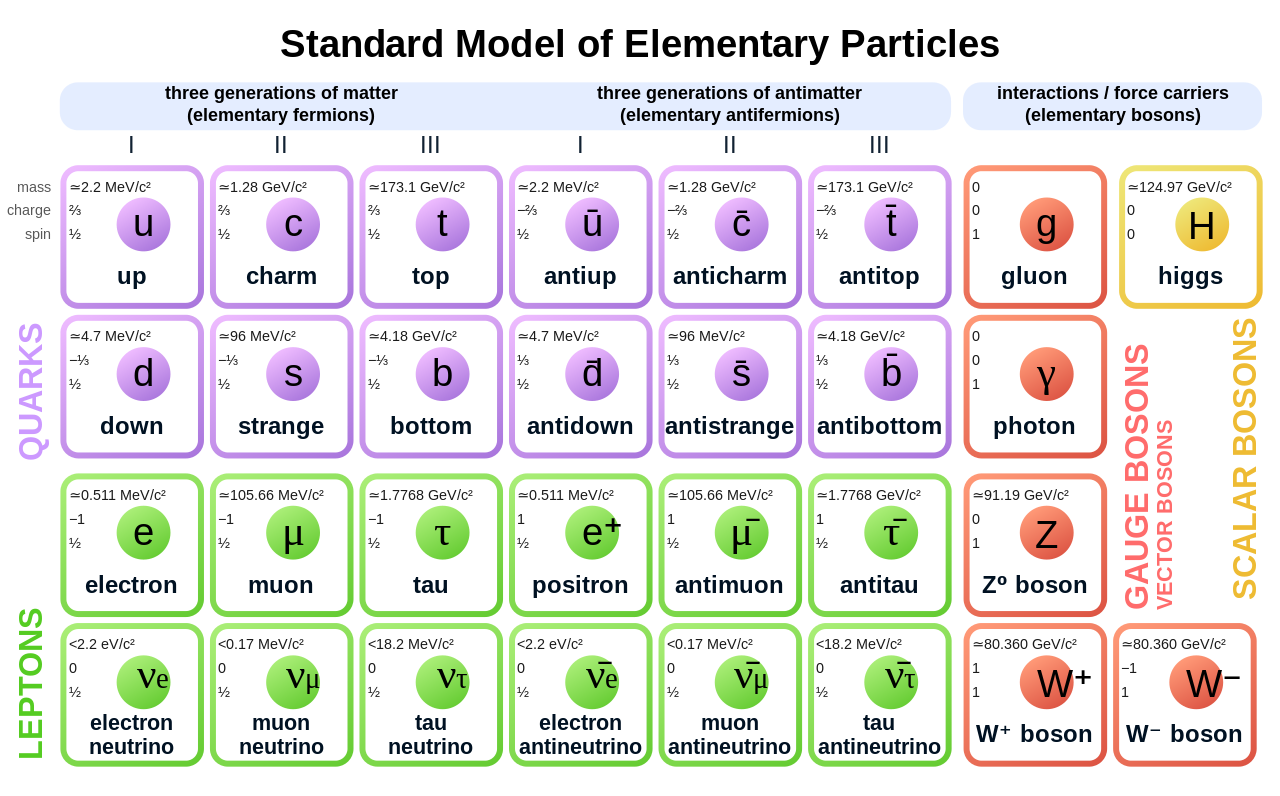
\includegraphics[width=\textwidth]{figures/Standard_Model_of_Elementary_Particles_Anti.svg.png}
    \caption{Fundamental fields in the Standard Model of particle physics}
    \label{fig:SM}
\end{figure}


The Standard Model represents today what early philosophy speculated almost 3000 years ago: the matter is composed by unbreakable elements and it is our quest as particle physicists to study the interactions that govern them.


\section{The role of LHCb in Standard Model testing}
Particle physics, as described by the Standard Model, has undergone extensive testing over the past five decades. The discovery of the third generation of quarks~\cite{E288:1977xhf, CDF:1995wbb} and leptons~\cite{PhysRevLett.35.1489}, in the experiments carried out in accelerators in the USA proved well the theoretical intuitions. The experimental evidence of force-carriers bosons such as the gluon~\cite{BERGER1979449}, W and Z bosons \cite{UA1:1983mne, UA2:1983mlz} were a triumph of the SM. At last, the  observation of the Higgs Boson~\cite{Aad_2012, Chatrchyan_2012} in 2012 marked a significant milestone, proving the SM predictive prowess and explanatory breadth. 

Despite its successes, the SM leaves several fundamental questions unanswered. These include the nature of dark matter, the absence of a quantum description of gravity, and the matter-antimatter asymmetry observed in the universe. In response to these lingering mysteries, the high-energy physics (HEP) community has embarked on a quest for New Physics (NP) phenomena that could provide experimental evidence for dynamics beyond the Standard Model (BSM). 

%Proposed BSM scenarios encompass SuperSymmetry (SUSY) models, leptoquarks, and extensions to the gauge boson sector, including the W’ and Z’ bosons.

Experimental tests of the SM unfold on different fronts.
For direct detection there are two pathways: 
the \textit{energy frontier} allow the production of new particles directly by increasing the energy available in the centre-of-mass system of the collider; the \textit{intensity frontier} notably searches the so-called Feebly Interacting Particles (FIPs), i.e. particles that are accessible with the available colliders but with small interactions that can not otherwise be detected.  
The \textit{precision frontier} searches instead indirect evidence of the existence of new particles or effects. This can be asserted studying subtle deviations from SM predictions through precision measurements. 

Flavour physics, with its unique capacity to detect effects of new particles contributing at loop level, has played a pivotal role in probing the SM structure. One enduring conundrum pertains to the organisation of fermions into three generations, both in the quark and lepton sectors, and the mechanism governing their mass hierarchy. Similarly, the structure of the CKM quark-mixing matrix remains a subject of investigation, alongside inquiries into the origin of the observed matter-antimatter asymmetry in the universe. In fact, according to the Big Bang theory, the universe should have produced equal amounts of matter and antimatter. However, our observations indicate that the universe is predominantly composed of matter. This asymmetry could have been generated in the violation of fundamental symmetries such as the charge conjugation $\mathcal{C}$ and parity $\mathcal{P}$. The $\mathcal{CP}$ violation suggests therefore that if a particle is replaced with its antiparticle and if its spatial coordinates are inverted, the laws of physics should change. 

There are three ways we can observe $\mathcal{CP}$ violation in particle physics experiment:
 \begin{itemize}
     \item Direct violation in decay: the probability of an initial state $M$ to decay into a final state $f$ is different than the probability of a $\mathcal{CP}$ state $\overline{M}$ of decaying into the final state $\overline{f}$;
     \item Violation in mixing: the transition of a particle $M^0$ into its antiparticle $\overline{M^0}$ is different than the inverse transition $\overline{M^0}\longrightarrow M^0$
     \item Violation in interference: a particle $M^0$ can decay directly into a final state $f$ or first oscillate into its antiparticle $\overline{M^0}$ before decaying. The overlapping probability amplitudes of these two pathways can interfere, leadind to observable $\mathcal{CP}$ violating effects.
 \end{itemize}
 
 The $\mathcal{CP}$ violation is incorporated into the Standard Model through complex phases in the CKM matrix for quarks and the Pontecorvo-Maki-Nakagawa-Sakata (PMNS) matrix for neutrinos mixing, a process analogous to quark mixing. The CKM matrix can be represented in the Wolfenstein parametrisation as 
 \begin{equation}
 V_{CKM} = 
     \begin{pmatrix}
         V_{ud} & V_{us} & V_{ub}\\
         V_{cd} & V_{cs} & V_{cb}\\
         V_{td} & V_{ts} & V_{tb}
     \end{pmatrix}
     =
     \begin{pmatrix}
         1-\lambda^2 & \lambda & A\lambda^3(\rho-i\eta)\\
         -\lambda & 1-\lambda^2/2 & A\lambda^2\\
         A\lambda^3(1-\rho-i\eta) & -A\lambda^2 &1
     \end{pmatrix},
 \end{equation}
 with $\lambda = \sin\theta_c$ (where $\theta_c$ is the Cabibbo angle) and $A,\rho,\eta$ real parameters.
 By representing the unitarity condition as $\sum_i V_{ij} V_{ik}$ for $j,k=d,s,b$ and $j\neq k$, we can define three triangles in the complex plane $\rho,i\eta$, as depicted in Figure~\ref{fig:unitary-triangle}.
 \begin{figure}
     \centering
     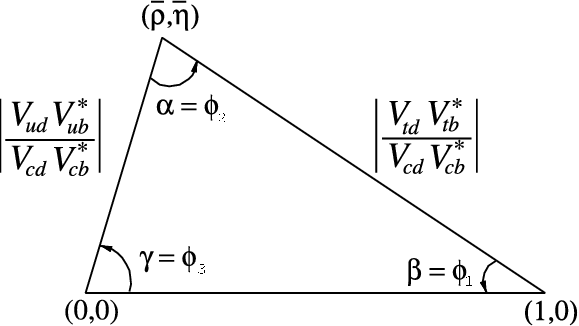
\includegraphics[width=0.5\textwidth]{figures/The-CKM-unitarity-triangle-Figure-from-Ref-4.png}
     \caption{Example of unitarity triangle in the complex plane  $\rho,i\eta$}
     \label{fig:unitary-triangle}
 \end{figure}
 In particular, the triangle for $j,k=d,b$ is non-degenerate, can better interpreted and measured. By measuring the angles and sizes of this triangle, we can make inference on the unitarity of the CKM matrix. If the relation is not proven unitary, this would mean the CKM picture of the weak interaction is incomplete, probing for NP effects not predicted by the SM~\cite{PhysRevLett.10.531, 10.1143/PTP.49.652}. 
 %If the measured sides and angles of the unitarity triangle do not align with expected results, it could signal new physics BSM.
 %Proposed BSM scenarios encompass SuperSymmetry (SUSY) models, leptoquarks, and extensions to the gauge boson sector, including the W’ and Z’ bosons.

Measurements of beauty and charm hadron decay rates and $\mathcal{CP}$ violation asymmetries offer opportunities for exploring physics beyond the SM, even at energy scales much higher than those directly involved in the processes. Notably, these observables, measured at the GeV scale, can probe mass scales ranging from $10^3$ to $10^4$ TeV, contingent upon the underlying structure of new interactions~\cite{Isidori_2010}. 

In this context, the LHCb experiment was conceived as one of the physics experiment aimed at studying $\mathcal{CP}$ violation and rare decays with the largest available samples of heavy hadrons. The LHCb detector is a single-arm forward spectormeter located in one of the collision point at the Large Hadron Collider (LHC) at CERN. In its acceptance, the cross section for $b$- and $c$-quark production reach respectively $\sigma_{pp\rightarrow b\bar{b}}\approx\SI{500}{\micro\barn}$ and $\sigma_{pp\rightarrow c\bar{c}}\approx\SI{2000}{\micro\barn}$~\cite{bCrossSection, Aaij:2057627}\footnote{At a center-of-mass energy of $\sqrt{s}=\SI{14}{\tera\eV}$}, allowing LHCb to observe the decays of a huge amount of $B$ and $D$ mesons. The tracking system comprehend the vertex locator (VELO), a sub-detector providing good spatial resolution ($\sim \SI{10}{\micro\meter}$) for reconstructing the decay vertices of these short-lived particles, while its robust particle identification systems, including two Ring Imaging Cherenkov (RICH) detectors, enable accurate discrimination between different particle types. A more detailed description of the detector will provided in Chapter~\ref{chp:experiment}, but these features among the others allow to perform precision measurements of quark-flavoured quantities.
%In contrast, direct searches for new states in other experiments at LHC are typically confined to mass scales in the TeV range, given 

%Precision studies of $\mathcal{CP}$ violation in elementary processes are crucial for understanding the cosmological matter-antimatter asymmetry. While the SM incorporates $\mathcal{CP}$ violation through the CKM matrix, ongoing efforts are dedicated to uncovering additional $\mathcal{CP}$-violating effects that may account for the observed matter dominance in the universe.

%\section{The LHCb physics programme}
%Given its potential to elucidate BSM effects, flavour phenomenology has emerged as a cornerstone of experimental particle physics. In this vein, the LHCb experiment was conceptualised and optimised to probe $\mathcal{CP}$ violation in b- and c-mesons, along with their decay rates and modes, providing precision measurements in quark-flavor physics for LHC at CERN.
The achievements of the LHCb experiment, leveraging data from Run~1 and Run~2, underscore its pivotal role in advancing the field of flavor physics. Notable milestones include the observation of rare decay modes such as $B^0_s\rightarrow\mu^+\mu^-$~\cite{PhysRevLett.111.101805}, observations of $\mathcal{CP}$ violation in the charm sector~\cite{Maccolini:2022y6}, and measurements of the CKM angle $\gamma$~\cite{Aaij_2016}, which can be obtained with high precision and carries negligible theoretical uncertainty. Additionally, LHCb has contributed to the discovery of exotic hadronic states~\cite{FANG202266, PhysRevLett.115.072001} and the measurement of various production cross sections in electroweak, QCD, and heavy-ion processes~\cite{ZBoson, Raab:2815873, Duan:2826531}.


%An intensity approach to particle physics -such as the one of LHCb- demands enormous datasets to improve the sensitivity of measurements. To achieve this, the LHCb experiment is undergoing significant upgrades~\cite{CERN-LHCC-2021-012} aimed at increasing data collection. This boost in data will enable tighter constraints on the parameter space of BSM theories. 

%With Run-3, the experiment is operating at an instantaneous luminosity that is five times higher than Run-2, achieving eventually a level of $\mathcal{L}=\SI{2e33}{\per\centi\meter\squared\per\second}$.

%The LHCb experiment has enhanced its capabilities thanks to Upgrade~I~\cite{lhcbcollaboration2023lhcb}, notably in its trigger and data-acquisition (TDAQ) system, as it will be later described in this thesis. 

%The LHCb Upgrade~II (UP2) programme~\cite{CERN-LHCC-2021-012} aims to make full use of the capabilities of a forward acceptance detector during the High Luminosity LHC (HL-LHC) operational period, scheduled to start in 2031. Foremost in the physics programme, are the possibilities of the experiment in its core areas of $\mathcal{CP}$ violation and rare decays in flavour physics.

%LHCb Upgrade II will be installed during Long Shutdown 4 (LS$4$), with operations beginning in LHC Run 5 which is scheduled to start in 2031. The experiment will operate at instantaneous luminosity of up to \SI{2e34}{\per\centi\meter\squared\per\second}, an order of magnitude above Upgrade I. LHCb will accumulate a data sample corresponding to a minimum of \SI{300}{\per\femto\barn}~\cite{Efthymiopoulos:2319258}. New attributes, installed in LS$3$ and LS$4$, will enhance the detector’s capabilities to a wider range of physics signatures. An overview of the LHC schedule is reported in Figure \ref{fig:LHC_schedule}.

%\begin{figure}
%    \centering
%    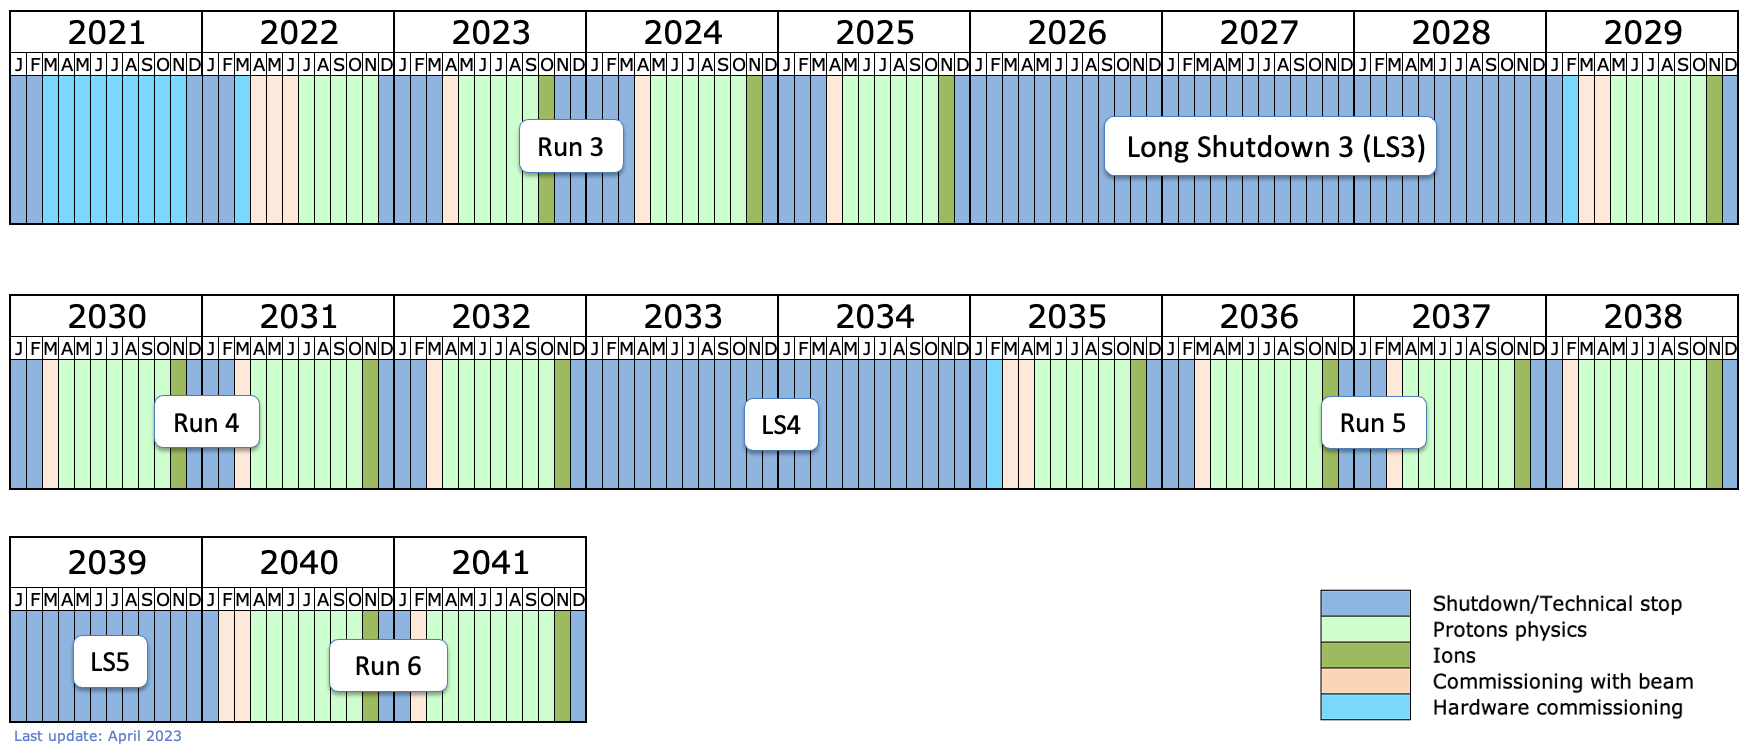
\includegraphics[width=\textwidth]{figures/LHC-long-term-Apr23.png}
%    \caption{The LHC long term schedule.}
%    \label{fig:LHC_schedule}
%\end{figure}

%The LHCb UP2 is being developed to lead the flavor physics research during the HL-LHC era. 
%In the SM, weak flavor couplings are not fixed, requiring experimental measurements to establish all matrix elements. However, the SM imposes constraints through the unitary nature of the CKM matrix, creating specific relationships among these elements that are commonly depicted as the \textit{unitarity triangle} in the complex plane. 
Moving towards the future, one of the main goal in the LHCb physics programme is the precise measurements of the unitarity triangle in the complex plane, testing the constraints of unitarity imposed by the SM. 
Although the measurement of the angle $\gamma$ currently has a 4-degree uncertainty~\cite{LHCb:2021dcr}, the collaboration expects to increase this precision by at least an order of magnitude. 

Another focus area is the $B_s^0$ weak mixing phase, with expectations to achieve a precision of approximately \SI{3}{\milli\radian}, on par with current indirect determinations based on the CKM fit.

The LHCb collaboration is also probing lepton universality, i.e. a prediction of the SM implying that the leptons $l$ interacts with gauge bosons with the same strength, differing only by their masses and lifetimes.
The investigation in new physics through lepton universality tests is carried out in semileptonic decays, such as in $b\rightarrow c l^-\bar{\nu}_l$ transitions. The plentiful semileptonic decays allow for precision studies of $\mathcal{CP}$ violation in $B^0-B^0_s$ mixing, with sensitivity to $\mathcal{CP}$ asymmetries reaching a few parts in $10^{−4}$. Similarly, the indirect $\mathcal{CP}$ violation in the charm system is projected to be very small, about $\mathcal{O}(10^{-4})$ in the SM, but the improved sensitivity of the experiment ($\mathcal{O}(10^{−5})$) that will be reached in Run~5 thanks to Upgrade 2~\cite{lhcbcollaboration2019physics} could increase the chances of observing this phenomenon. Additionally, a comprehensive program of direct $\mathcal{CP}$ violation searches in charm is planned, examining both new physics and Standard Model-sensitive modes.

%The LHCb Upgrade II will continue the significant impact of the experiment on hadron spectroscopy, enabling detailed studies on known states and the potential discovery of new ones. Pentaquark multiplets, beauty-containing pentaquarks, and doubly charmed tetraquarks are among the fascinating targets with the enhanced data from this upgrade.



\section{Pushing the real-time frontier}
For the ongoing LHC Run~3, LHCb has introduced an innovative trigger system based on the full software reconstruction of every collision event. In this new configuration, the entire event is reconstructed in detail at full resolution in real time at the collision rate, allowing for a higher specificity for the selection of the events. This marks the first time that a \SI{40}{\mega\hertz} stream of LHC collision events is filtered based on offline-quality event reconstruction performed in real time. This implies processing a flow of~$\sim 40$~Tbits/s, which poses a significant computational challenge. 

The computing infrastructure utilised by HEP experiments has traditionally leaned heavily on general-purpose CPUs, which are widely accessible and have historically seen performance gains driven by increasing clock frequencies. However, the slowdown of Moore's law since the early 2000s~\cite{Tuomi_2002}, coupled with the increasing demands of the physics landscape necessitating higher precision measurements, has prompted a shift towards specialised solutions to tackle the escalating computational demands posed by experiments. Heterogeneous computing, which integrates computing machines with diverse architectures within the same workflow, offers a strategic approach to optimising performance by assigning tasks to the most appropriate architecture based on their inherent characteristics. This often involves pairing conventional general-purposes CPUs with specialised co-processors, such as GPUs or FPGAs, to leverage their unique capabilities in accelerating specific computations and enhancing overall efficiency.

For the renewed trigger system, the LHCb collaboration has decided to pursue the path of heterogeneous computing. The initial data selection in past LHCb runs was based on a ``level-zero" trigger, based on rough measurements of calorimetric energy deposition and muon detector activity. This has been replaced in the current Run~3 by a HLT1 system based on an array of $\sim 500$~GPUs embedded in the hardware structure of the event builder system operating in parallel on different events. This parallelisation allows to take a first-level decision on events to be kept for further analysis. This decision is taken immediately after the event building and is based on fully reconstructed event quantity. Events selected at this level are then further processed and selected by a system based on commercial CPU servers. Beside enhancing discriminating power for the selection of events of physics interest, this new paradigm allows at once to greatly reduce the data stream moved from the event builder system to the CPU servers. 

%LHCb installed a new TDAQ system in Upgrade I~\cite{lhcbcollaboration2023lhcb}, designed to process events in real-time at a offline quality level.  necessitates the adoption of heterogeneous computing solutions. By harnessing diverse computing architectures, such as GPUs and FPGAs, LHCb aims to tackle the formidable computational challenges posed by track reconstruction and event selection at the unprecedented collision rates of LHC..

%In Run 3, LHCb introduces an innovative trigger system, marking the first time that all collision events at the LHC undergo a real-time and offline-level quality reconstruction, operating at an average frequency of \SI{30}{\mega\hertz}. This decision arises from the need for detailed and flexible trigger selections crucial for the physics events targeted by LHCb. Reconstructing events at this frequency, especially tracks, poses a significant computational challenge. To address this, LHCb adopts a heterogeneous computing system. In this setup, the initial trigger level (HL$T1$) relies entirely on an array of GPUs, leaving CPU resources for the subsequent level (HLT$2$), where thorough event reconstructions occur at a reduced rate compared to HLT$1$. 


However, even if these technologies can grant faster operations thanks to higher performances and parallelisation, much of the computing time is spent performing low level and repetitive tasks, such as tracking reconstruction and clustering of particle hits on the detector. These processes in Run~3 are well-handled by the GPUs that multiplex the information of different threads, enabling parallel computing.

As LHC moves its schedule to future runs, the collaboration plans to increase the operational luminosity by another order of magnitude compared to Run~3, making it hard for these kind of reconstruction tasks to keep pace. With Run~5 planned to start in 2035, LHCb will reach a pile-up multiplicity -- i.e the mean number of interactions per bunch crossing -- of $\mu\approx 40$ generating more than 2000 tracks, as depicted in the simulation of Figure \ref{fig:velo_pile-up}. 

\begin{figure}
    \centering
    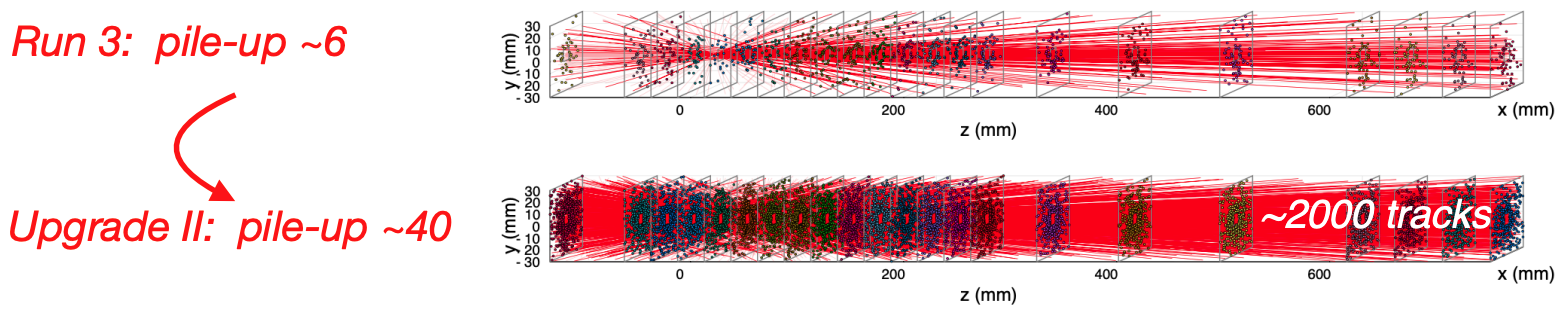
\includegraphics[width=\textwidth]{figures/VELO_pile-up.png}
    \caption{Simulation of hits and tracks generated by different pile-ups. In the upper one the actual situation is depicted, with a pile-up of $\mu\approx 6$, while in the other the one expected for Run~5, planned to start in 2035.}
    \label{fig:velo_pile-up}
\end{figure}

The scenario foreseen for Run~5 requires the collaboration to develop new strategies to process the data, in order to perform the event reconstruction in real time. One proposal for Run~5 is to implement the reconstruction of some quantities to an earlier stage of the trigger chain, encompassing  more complex information -- called primitives -- directly in the readout of the detector before the complete event is assembled by the event builder. The RETINA~\cite{refId0} R\&D project for instance aimed at moving the track reconstruction at the readout level. This step would completely change the way events are assembled in the trigger chain, which would handle already reconstructed tracks instead of raw hits on the detector. In this context, RETINA has emerged with a focus on implementing an FPGA-based computing architecture inspired by visual processing. Using a pipelined internal architecture, certain operations are executed swiftly ``on the fly" for all hits detected in each event, without causing delays in data acquisition or requiring extensive computational resources, provided the firmware is appropriately designed. Notably, this efficiency is maintained despite an average hit rate of approximately $4 \cdot 10^{10}$/s, which may appear prohibitive for exhaustive processing.
This would be indeed extremely advantageous, saving computing power and freeing the CPU farm of redundant and time-consuming tasks. This would allow to make full exploit of CPU time and computing power that can be devoted to higher level tasks in physics selection, where the flexibility of general-purpose CPUs and their associated high-level software environment is actually well employed. The LHCb collaboration has decided to pursue this approach starting in Run~4, with the introduction of a dedicated FPGA system for real-time tracking in the forward region~\cite{Morello:2888549}.

In the context of this further evolution of the approach, I propose the reconstruction of additional primitives, allowing a \textit{real} real-time analysis of some physical quantities. The emphasis on the \textit{real} adjective is due to the fact that this reconstruction matches the collision throughput of \SI{30}{\mega\hertz} and does not multiplex the information on a set of GPUs as it currently implemented in Run~3.

The objective of this thesis work is to further exploit the real-time accessibility of all hits from a complex detector at LHC, i.e. to extend the exploration potentials of real-time FPGA reconstruction. In particular, in this thesis I implemented three different estimators that enable the estimation of three quantities in real time:
\begin{itemize}
\item instantaneous luminosity;
\item luminous region position at the LHCb interaction point;
\item movements of the VELO sub-detector.
\end{itemize}

The idea to perform some tasks of the reconstruction sequence at earlier stages of the data acquisition chain is not only relevant to enhance the computing performances of the high-level processing farm of the LHCb experiment, but it also advances a new paradigm in HEP experiments. 

As it will be described in the thesis, a new direction in real-time reconstruction has thus established, for which the output data from a detector would no longer be raw data, but they would be well-reconstructed primitives e.g. tracks or reconstructed particle hits.
 

\section{An immediate motivation of the monitoring tasks}
This thesis aims to explore the wider potential of a new approach to HEP data processing, that might in the future become widely used, in which pre-reconstructed data is available at a very early stage in the data acquisition chain. This is the case that LHCb will face from Run~5, in which the reconstruction at early stage will be crucial to allow data-taking at higher accelerator luminosities. However, some recent problems in the experiment highlight applications that could help some challenges that LHCb is facing in the on-going Run~3.


In the latest years misalignment and drifting movements of the VELO have limited the precision of important measurements, such as the precise determination of the $B_S^0-\overline{B_S} ^0$ oscillation frequency, where the parameters concerning VELO alignment represent the major contribution to the systematic uncertainty~\cite{b0b0soscillation}. The need for a faster and more frequent alignment procedure is therefore strongly felt.  
    
Currently, the alignment and calibration phase of LHCb takes place within the DAQ as part of Real-Time Analysis workflow, as it will be better described in Section \ref{sec:alignment}. Specifically, the alignment of the VELO occurs between HLT$1$ and HLT$2$ by minimising the $\chi^2$ of all tracks with respect to alignment parameters $\alpha$ computed from the residuals of the tracks. The alignment parameters $\alpha$ are then fed back to HLT$1$ for a new improved track fitting, which in turn refines the estimation of $\alpha$. This iterative procedure is repeated until a convergence in $\alpha$ is achieved~\cite{FRUHWIRTH1987444, Frühwirth:803519}. As this process relies on reconstructed tracks, the selected events must be buffered in the Event Filter Farm, resulting in potential delays of hours or even days before alignment is performed. Furthermore, alignment is executed only once per run\footnote{A LHCb run corresponds approximately at 1 hour of data-taking}, thus movements of the VELO within the same run are not considered~\cite{Dziurda:2640712}. In contrast, the estimator discussed here offers the capability to determine the two VELO halves position with notable precision in real time. This real-time capability contrasts with the current alignment method, providing immediate feedback and the potential to address alignment issues promptly during data collection.

The reconstructed luminous region positions are a valuable input for the reconstruction algorithms of primary vertices (PVs). As this thesis work was started, the vertex fitting algorithms relied on a hardcoded parameter for the luminous region position, followed by an iterative refinement procedure. However, this iterative method is computationally demanding. Alternatively, supplying the vertex fitting algorithm with a real-time estimation of the luminous region could accelerate the process. Since the beginning of this thesis work, different attempts have been made in LHCb for providing this quantity to the reconstruction algorithms, with mine being one of them. Integrating my estimator into these algorithms could significantly accelerate and increase the efficiency of the PV finding process by providing updated luminous region position inputs. 

Furthermore, the current luminosity estimation provided by the official luminometer PLUME suffers from non-linearities. This deviation from the expected linear behaviour could bias the luminosity measurement and therefore affect the precision of cross-section measurements. The estimation of the luminosity proposed in this thesis proved linear and robust, providing an effective complement to the PLUME measurement.

Finally, luminous region shifts affect every luminosity measurement, independently from the tool used for the estimation. The luminous region estimator implemented in this thesis can effectively address these shifts and provide corrections for online luminosity measurements, which are known to depend on the luminous region position. By incorporating the estimator into the luminosity measurement process, we can mitigate the impact of luminous region shifts and enhance the accuracy of online luminosity measurements.
